\documentclass[12pt, final]{article}

%%%%%%%%%%%%%%%%%%%%%%%%%%%%%%%%%%%%%%%%%%%%%%%
\usepackage{virgil_env} %% Import the Virgil environment
\usepackage{multirow}
\usepackage{fullpage}
\usepackage{nips10submit_e}
\usepackage{afterpage}
\usepackage{cite}
\usepackage{caption}
\usepackage{subfigure}
%\usepackage{subfig}

%\usepackage{subcaption}
\nipsfinalcopy
%\input{this_symbols.tex}  %% symbols for this paper


\usepackage[utf8]{inputenc}


\graphicspath{{./}{figs/}}
\usepackage{booktabs,multirow,nicefrac}

\usepackage{xspace}
\usepackage{float}


\usepackage{listings} % to make pretty code


\usepackage{tabu}% http://ctan.org/pkg/tabu

\newcommand{\dashrule}[1][black]{%
  \color{#1}\rule[\dimexpr.5ex-.2pt]{4pt}{.4pt}\xleaders\hbox{\rule{4pt}{0pt}\rule[\dimexpr.5ex-.2pt]{4pt}{.4pt}}\hfill\kern0pt%
}
\newcommand{\rulecolor}[1]{%
  \def\CT@arc@{\color{#1}}%
}

\newcommand{\tt}[1]{{\texttt{ #1 }}}
\newcommand{\fname}[1]{ \operatorname{ #1 } }
\newcommand{\opname}[1]{ \operatorname{ #1 } }
\newcommand{\opcode}[1]{\textsc{\texttt{#1}}}


\usepackage{authblk}
\author{Virgil Griffith}
\author{???}
\author{Vitalik Buterin}
\affil{Ethereum Foundation}


%%%%%%%%%%%%%%%%%%%%%%%%%%%%%%%%%%%%%%%%%%%%%%%%%%%%%%%

\bibliographystyle{plos2009}

\usepackage{mathenv}
\usepackage[]{algorithm2e}


\title{Blockchain Resource Pricing}

%%%%%%%%%%%%%%%%%%%%%%%%%%%%%%%%%%%%%%%%%%%%%%%%%%%%%%%%%%%%%%%%%%%%%%%%%%%%%%%%%%%%%%%%%%%%%%%%

%%%%%%%%%%%%%%%%%%%%%%%%%%%%%%%%%%%%%%%%%%%%%%%%%%%%%%%%%%%%%%%%%%%%%%%%%%%%%%%%%%%%%%%%%%%%%%%%


\begin{document}

\maketitle
\vspace{-0.2in} \TODO{\today}

%{\centering {\sffamily \today} \vskip10pt }

%\vspace{-0.2in} {\centering \today } \vspace{0.1in}



%\vspace{-0.05in}
\begin{abstract}
\todo{this will be reworked at the end} Resource pricing continues to be one of the most interesting and difficult challenges in blockchain protocol design. Blockchains are a classic example of the ``tragedy of the commons'' problem, where users have the ability to send transactions that require all full nodes in the network to expend resources on transmitting transaction data, processing transaction execution, and storing the transaction and the results of its execution. If left unpriced, massive overconsumption of these resources is likely to result, making it quickly infeasible to run a node or otherwise participate in maintaining the network.

In such cases, economic theory generally dictates pricing the resources in question, and setting the price to equal the social cost that the act of consuming each resource imposes on the network. However, the heterogenous nature of the resources involved, the large portion of the social cost that exists in the form of intangible and difficult-to-value harms such as centralization risk, and the need to create an automated algorithm that can set prices in a wide range of future scenarios without human intervention all make it very difficult to set prices that are optimal.

It may well be the case that the best we can do is not a first-best or even a second-best result, but rather creating price-setting formulas that do not lead to extremely undesirable outcomes when faced with situations that are unexpected.
\end{abstract}

%%%%%%%%%%%%%%%%%%%%%%%%%%%%%%%%%%%%%%%%%%%%%%%%%%%%%%%%%%%%%%%%%%%%%%%%%%
\section{Introduction}
%%%%%%%%%%%%%%%%%%%%%%%%%%%%%%%%%%%%%%%%%%%%%%%%%%%%%%%%%%%%%%%%%%%%%%%%%%

We discuss a platform where users send transactions (cryptographically signed messages representing actions), and these transactions get bundled into blocks by randomly assigned ``validators'' drawn from a set of consensus-participating nodes (e.g., proof-of-work block miners or proof-of-stake block proposers), which we will generically call ``validators''; for each block, validators are randomly assigned but may include whatever transactions they wish into their block.\footnote{Though the protocol may set limits on the number or type of transactions to be included.}. We define the sequence of blocks that the validators collectively generate as a \emph{blockchain}.

There exists a ``state transition function'' $\fname{STF}(state, tx) \rightarrow state^\prime$, which takes a state, and a transaction, and returns a new state (e.g., Using a very simple example, from the pre-state ``Alice has 20 coins, Bob has 40.'', and a transaction ``Alice sends 10 coins to Bob'', the post-state would be ``Alice has 10 coins, Bob has 50.''); the ``current state'' of a blockchain refers to the result of taking some commonly agreed ``Genesis state'' and sequentially processing each transaction in every block (that is, if there's been $m$ transactions since the Genesis state, $s_0 = \fname{GENESIS}$, $s_1 = \fname{STF}(s_0, tx_1)$, $s_2 = \fname{STF}(s_1, tx_2), \ldots, s_m = \fname{STF}(s_{m-1}, tx_m)$).

A ``validator'' is defined as any agent who maintains a record of the current state.  A ``full validator'' (a.k.a. ``full node''), is a validator who maintains a record of the \emph{complete chain} since the Genesis block.  Every full validator continually downloads each block in sequence and process its list of transactions to update their view of the current state.

There are three (mutually exclusive) distinct types of nodes, they are: validators, passive full nodes, and light clients.  Of these, ``full nodes'' is the union of all validators and passive nodes.  And ``nodes'' is the union of validators, passive full nodes, and light clients.  In our analysis we are chiefly concerned with \emph{full nodes}---they are the ones who are burdened by publishing blockchain transactions.


The above suffices as a description of a blockchain for the purpose of this paper. Resource pricing challenges are generally independent of any specific consensus mechanism.  And from the above, we see that a user sending a transaction imposes four of costs on the blockchain's validators:

\begin{itemize}
\item[] \textbf{Bandwidth cost:} the cost of all nodes downloading each submitted transaction, bundling it into a block, and then rebroadcasting the transaction as part of some block.  For $n$ nodes, this download and and then rebroadcast cost scales $\Theta(2n) = \Theta(n)$.

\item[] \textbf{Computational cost:} the cost of every node executing the state transition function for the transaction.  For $n$ nodes, this cost scales $\Theta(n)$.

\item[] \textbf{History storage cost:} the cost of indefinitely storing the transaction for all nodes that store the blockchain's full history.  For $n$ storing the full history, this scales $\Theta(n)$.

\item[] \textbf{State storage cost:} the execution of the state transition function for the transaction may increase, decrease, or have no impact on the size of the state. If the transaction increases the state size, this imposes a cost on all full nodes---even those that discard history, as having the state is necessary to validate the next block.  For $n$ full nodes, this cost scales $\Theta(n)$.
\end{itemize}

These four costs manifest themselves in two ways. The first and simpler cost to understand is that every transaction imposes an economic burden on both validators and even non-validating nodes.  This economic burden of electricity, bandwidth fees, and hardware costs can be viewed as a simple externality. The second and more subtle cost is that any of these costs may lead some nodes to decide that it is too burdensome to be a full node, and instead elects to be a light node, use a centralized service\cite{infura}, or join a centralized mining/stake pool. This is considered a systemic risk, because if the network rests on only a small number of full nodes then it will be easier for those nodes to collude to change the protocol in disagreeable ways.


\section{Prior Work}

In Ethereum, resources are priced using a simple ``cap-and-trade'' scheme. A metric is defined for the magnitude of resources or ``weight'' that a transaction consumes, and there is a protocol-defined maximum total weight a block may contain. Validators have free rein to select transactions as long as the total weight of the block is below that limit. An equilibrium is established where users attach fees to their transactions which go to the validator that includes the transaction in a block, and Rational validators select the transactions paying the highest fee per unit weight.

%For Bitcoin, the total weight is simply the size in bytes of the serialized block, with a maximum weight of 1,000,000;\footnote{In the specific case of Bitcoin, the weight is in ``bytes'', we generalize this to ``weight''.} but we  a proposal called ``segregated witness'' \cite{bip:141} changes the weight function to, 

%\begin{equation}
%\fname{weight}(block) =  4 *\tt{num\_bytes\_of\_nonsignature\_data} + \tt{num\_bytes\_of\_signature\_data} ,
%\end{equation}
%\todo{Put description here of signature vs nonsignature data.}
%with a maximum weight of 4,000,000 per block.

In Ethereum, there is a measure called ``gas'' which incorporates the size of the block as well as the computational cost of executing the state transition function on every transaction therein.  This can be usefully approximated as,

\begin{equation}
\fname{weight}(block) = 68* \tt{num\_bytes} + 3* \tt{num\_computation\_steps} \; , 
\end{equation}

though the gas function is in reality much more complex (See Appendix \ref{appendix:gasfunction}. There is a per-block gas limit, which validators can vote on (every validator can ``upvote'' or ``downvote'' the gas limit by a maximum of $\sim\!0.1\%$), and currently most validators are voting for a gas limit of $\sim \! 4$ million. \todo{cite}

The main problem is that apriori it has been difficult to determine a reasonable weight limit.  Moreover, it is difficult to predict how the validators will respond to changes in weight limits, technology, or user preferences, and any early limit may easily end up too small or too large. A blockchain community can mitigate this risk by exercising a willingness to continually adapt parameters (or, as Ethereum does, let validators vote on some of the parameters or including a difficulty bomb\cite{wood2014ethereum} that ensure ongoing hard forks), and only setting limits in stone only after there's battle-tested economic theory underpinning these choices.

However, in the very long term, even the most carefully set limits may be unsatisfactory, and the time between hardforks can be lengthened by carefully reasoning about the economics beforehand.


\section{Pricing Resources under Uncertainty}
\label{sect:uncertainty}
Blockchain resource pricing has many parallels to regulatory responses to environmental pollution.  Particularly, although the validator of a block is compensated for publishing the transactions, the cost of that block being published is borne by \emph{all full nodes}.  This cost being born by all full nodes is the negative external we wish to limit.  Both use economic interventions to limit activities with negative externalities, where the negative externalities have both measurable components as well as components with high Knightian uncertainty (i.e., ``unknown unknowns'') \cite{knight1921risk}.  Many results from environmental economics \cite{barder14} are directly applicable to blockchains.

For example, Weitzman's 1974 paper ``Prices vs Quantities'' \cite{weitzman1974prices}, outlines the tradeoffs between regulation by price (e.g., carbon taxes) versus regulation by quantity (e.g., issuing a fixed number of permits and letting them trade on the market). If the policymaker has perfect information, the two are, on average, equivalent: for any desired price, one can choose an equivalent quantity-based policy by issuing exactly the number of permits equal to the equilibrium quantity at that price. However, when there is uncertainty about the position and shape of the cost-benefit curves, the two approaches have substantial differences.

Consider a world where the social cost (negative exeternalities) of consuming a resource is fixed, but the less you consume the private cost increases rapidly. If you, the policymaker, set a quantity limit too low, then consumers pay extraordinate private costs from nonconsumption.  But if you instead set a price, then the combined damage (social + private costs) from such a miscalculation is much lower.

If on the other hand, the \emph{private} cost of abstaining is fixed yet social cost of consumption increases rapidly, then setting a price is riskier. For example, consider a scenario where the social cost of consuming $<1,000$ resource units is acceptable, but going above 1,000 risks disastrous consequences (e.g., some ``tipping point'' theories of global warming\cite{wiki:runaway}). The marginal social cost \question{ecosystem damage?} when people consume 1,050 resource units will be much higher than if they consumed merely 900.  In this case, if you set a price targeting 900 consumed resource units, but you underestimated the demand, then the equilibrium quantity may exceed 1,000, with perilous consequences.  In this case, if you simply issued 990 permits, and let them trade on the market, then this risk is mitigated.


\begin{figure}[ht]
\centering
\subfigure[]{
	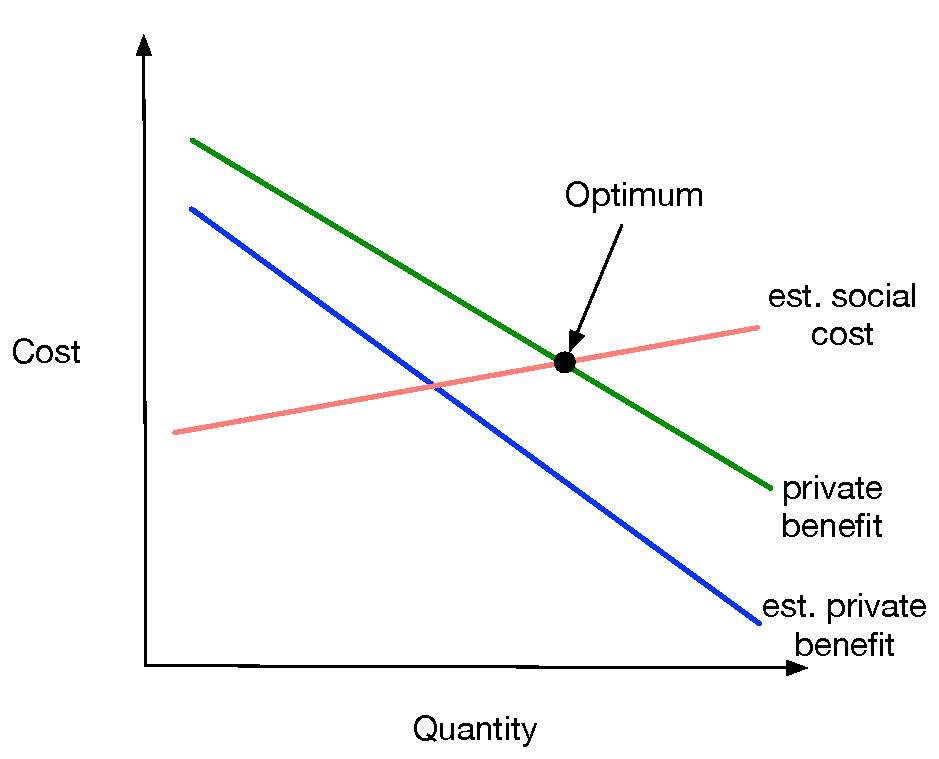
\includegraphics[width=3in]{fig1a.pdf}
%    \label{fig:1a}
}
\subfigure[]{
	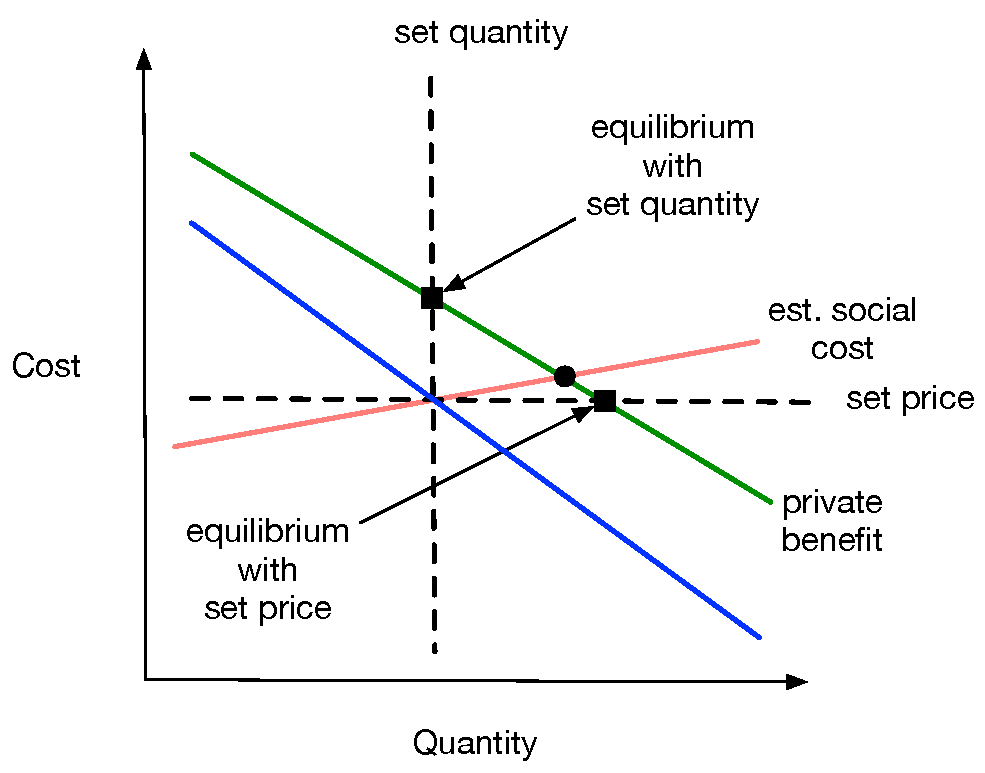
\includegraphics[width=3in]{fig1b.pdf}
%    \label{fig:1b}
}

\subfigure[]{
	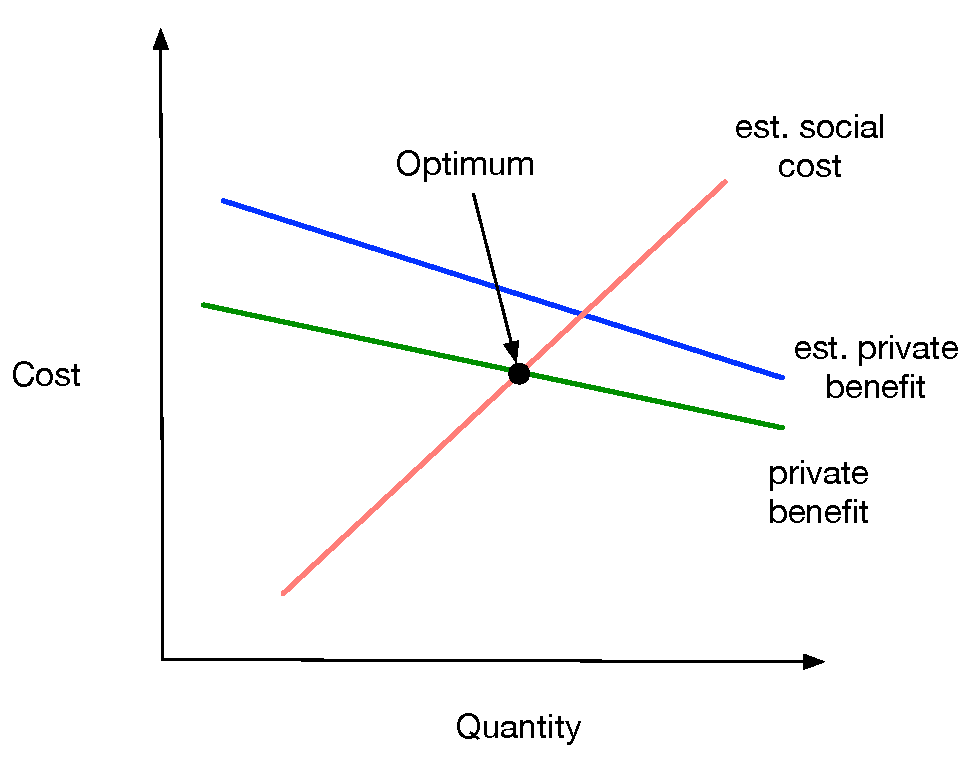
\includegraphics[width=3in]{fig1c.pdf}
%    \label{fig:1c}
}
\subfigure[]{
	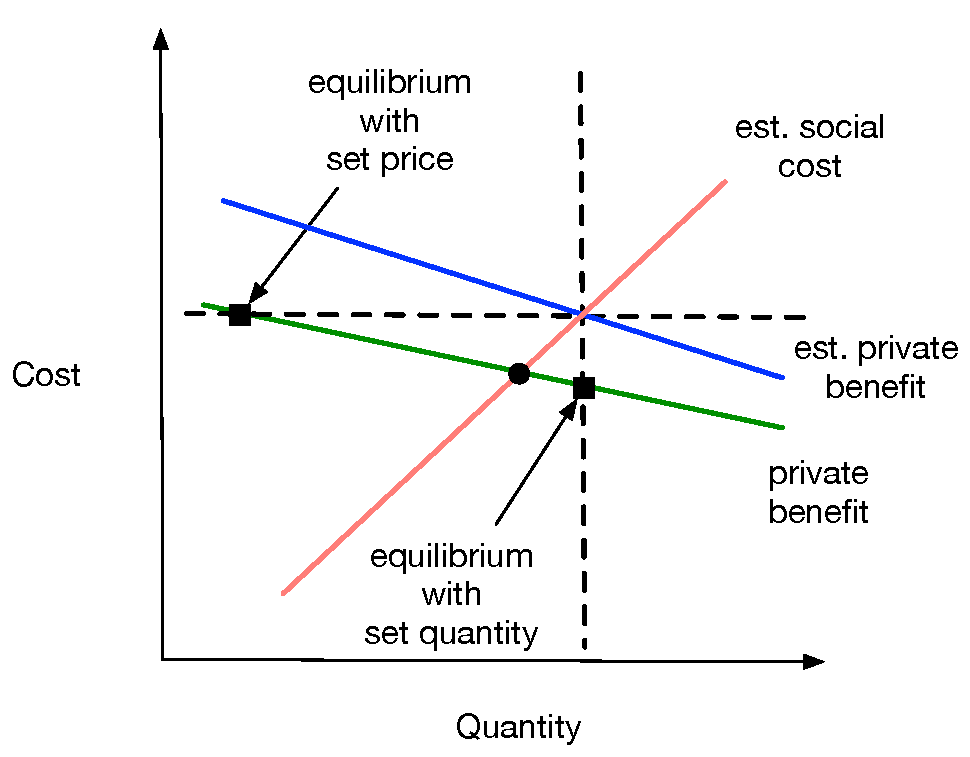
\includegraphics[width=3in]{fig1d.pdf}
%    \label{fig:1c}
}
\caption{Figures (a)--(b) show the first scenario in which it's better to set a price.  Figures (c)--(d) show the second scenario where it's better to set a quantity.}
\label{fig:one}
\end{figure}




Taken together, if the consumer's private costs increase faster with quantity than the \todo{aggregate?} marginal social costs, then setting prices is better.   But in the other case setting the quantity is better, or equivalently,


\begin{equation}
\frac{ \fname{cost\_to\_consumer}^{\prime \prime}( \opname{quantity} ) }{ \fname{cost\_to\_others}^{\prime \prime}( \opname{quantity}) }  > 1 \; ,
\end{equation}

then set prices.  Otherwise set quantity.  We use the second derivitive because we are specifically talking about the \emph{the rate of change} in marginal costs.  \todo{replace the above using Leibniz notation.} 


The argument above applies only if costs and benefits are independent. If changes in the cost and benefit curves are correlated, then an additional term must be added into the choice rule, increasing the relative attractiveness of limiting quantity. \new{To see this intuitively, consider the extreme case where uncertainty in cost and benefit is perfectly correlated; in such a scenario, if original estimates of cost and benefit prove incorrect, both curves will move up or down in lockstep, and so the new equilibrium will be directly above or below the original estimated one; hence, a quantity-targeting policy would be perfectly correct and a price-targeting policy would be pessimal.} This analysis covers only two possible policies, but a much greater space of options is available.  One can think of policy space as the space of possible supply curves for a given resource, where a pricing policy represents a horizontal supply curve and a cap-and-trade scheme represents a vertical supply curve. Various forms of diagonal supply curves are also possible, and in most cases some form of (possibly curved) diagonal supply curve is optimal.\footnote{ostrom2002}

In applying these policies to designing blockchain protocols, there are several complicating constraints: 

\begin{enumerate}
\item All price-based policies must be denominated in the base cryptocurrency (e.g., bitcoin (BTC), or ether (ETH)), and such cryptocurrencies are very volatile. Analyzing in terms of ether, there is a high level of uncertainty in both the benefit and cost curves; a 10x price rise of ether effectively implies that the cost and benefit curves both fall by a factor of ten. Of course, one can argue that such a price rise would be caused by an outside factor (e.g., ``increasing adoption'') that then also shifts the benefit curve upward (by introducing new users some of whom would be willing to pay more than some existing users) and shifts the cost curve upward (because the security of the blockchain becomes more valuable); however, regardless of the exact net balance of these factors, it is clear that unexpected changes in benefit and cost are very likely positively correlated---a fact which, as mentioned above, motivates a preference toward quantity-based approaches.

\item It is difficult to tell whether the cost curve is increasing, flat or even decreasing.
An intuitive argument for the claim that the cost curve is increasing would be, ``It's clear that the blockchain can handle 2MB blocks, but anything beyond that brings great risk of the protocol becoming very centralized and so it is best not to go there''. An intuitive argument for the claim that the cost curve is decreasing would be, ``It's clear that the increase in centralization-risk resulting from increasing the maximum block size from 1 MB to 2 MB is greater than the centralization-risk from going from 100 MB to 101 MB''. In reality, the cost curve may be nigh flat, or it may even be an S curve, for example the added centralization risk per byte increasing between 1 MB and 10 MB but then decreasing beyond that. In general, these arguments suggest price-based approaches.

We can start by estimating the cost-benefit curves. Let's start with the cost curve. A 2016 study\cite{cornell-position} estimated as a function of blocksize the proportion of bitcoin full nodes that will be able to dowlnload the entire block before the next appears.  The results are in \figref{fig:two}.  Now, we can combine these measurements with a crude cost function: each $2x$ reduction in the number of full nodes costs one point of utility. In general, cost functions (and utility functions more generally) are a matter of the values of the users of the system, and so one cannot ``prove a utility function correct''; however, we can try to intuitively justify our choice. In this case, we can claim that, in terms of centralization risk, the difference between 100 nodes and 200 nodes feels similar to the difference between 1000 nodes and 2000 nodes, and the difference between 2000 nodes and 2100 nodes feels insignificant by comparison. If one interprets the social value of full node count in terms of coordination costs \cite{vitalik-coord}, then one can argue that the average ``social distance'' between two nodes out of N that would need to coordinate is $\sim \log(N)$, and the difficulty of overcoming the coordination problem is proportional to this.  We can convert the above chart into a new chart based on utility reduction:
\end{enumerate}


\begin{figure}[hbt]
\centering
\subfigure[Functional full nodes as function of blocksize from \cite{cornell-position}]{
	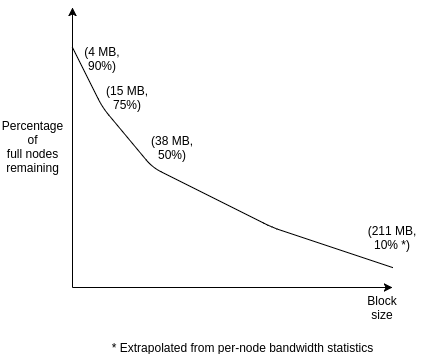
\includegraphics[width=3in]{blocksize_fullnodes.png}
%    \label{fig:1a}
}
\subfigure[Drop in utility]{
	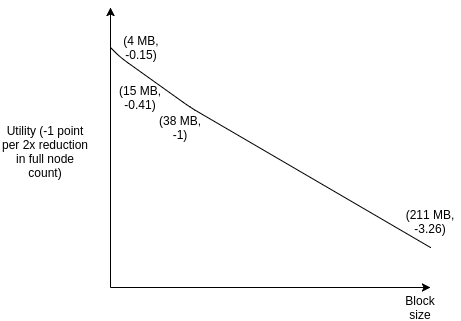
\includegraphics[width=3in]{blocksize_disutility.png}
%    \label{fig:1b}
}
\caption{Estimating the utility}
\label{fig:two}
\end{figure}




Another way of looking at the cost of including transactions is the fact that larger blocks take longer to propagate through the network, and the unfairness that arises because well-connected validators are less likely to create outdated blocks than more peripheral vlaidators. The probability of blocks not getting included in the chain also increases $\Theta(n)$ with block size that in the long term slowly decreases because of improvements to technology \cite{vitalik-uncle-rate}.

There is one argument that the marginal social cost of a transaction increases should under high load: if the current transaction load is much higher than the recent average, then there is a greater risk that these transactions are part of a denial of service attack, and so the expected social cost is slightly higher.  There are plenty of legitimate reasons why transaction spikes could happen, such as Ethereum-based token sales \cite{medium-codetract}.

Hence, there is fairly little evidence that of the marginal cost of a transaction increases with the existing load, and there are also limited arguments and evidence to suggest that the marginal cost of a transaction is decreasing. In either case, under a simple model of cost/benefit uncertainty this suggests, at first glance, that block size / gas limits are the worst possible ways to regulate blockchain resource consumption, at least out of the possibilities that could reasonably be employed. \question{didn't quite understand this.}

\subsection{Estimating the Private Benefit Curve} 

The private benefit curve, the demand for sending transactions, is hard to estimate. We can make a crude model where we assume that the private benefit curve is a power law with some constant elasticity $k$---that is, if transaction fees are reduced by a factor of 2, then the number of transactions sent will increase by a factor of $2^k$. We can then add to the model an assumption that the demand curve, denominated in the native currency, is increasing exponentially at a constant rate. We then try to fit parameters to minimize total squared error. \todo{The power law isn't a standard demand curve.  Ideally, we'd like to determine the demand curve from mining \emph{empirical data}.}

Extrapolating into new regimes is a common source of error, but without better guidance, this analysis roughly says: ``Before Bitcoin blocks were full, block sizes were increasing $X\%$ per month. After Bitcoin blocks got full, fees started increasing $Y\%$ per month. Therefore, we estimate the elasticity at $Y / X$''. \question{Is there anything better we can do than this estimate?}

The best-fit for a set of data given by Blocktrail [cite] is an elasticity of 0.275---that is to say, decreasing fees by $2x$ will increase usage by only $\sim 21\%$, and alternatively doubling the block space will decrease fees by a factor of $\sim12.4$. If we weight the error function so that the most recent run-up in fees in the last 6 months is counted triple (this can be justified by saying that the last 6 months represent a distinct ``phase'' that is shorter, but equal in importance, to the previous 18), then the best-fit elasticity drops to 0.2. However, the margin of error is wide: elasticities as high as 1.05, and as low as 0, get error values less than twice as high as the optimum.   \question{It's unclear how these were gotten from Blocktrail.  I don't see this in their data.}

Additionally, it is important to note that this only measures the short-term demand curve looking at actions taken over a few months and not taking into account longer-term adjustments that could happen in the market only after a couple of years; in the real world, for example, it is an established fact that long-run elasticity of gasoline is higher than short-run elasticity\cite{env-econ}; and so this is likely true with Bitcoin transaction fees and Ethereum gas as well. \question{Don't quite understand this.}





------------------

\section{Cryptocurrency Prices}

However, the simple model in \figref{fig:one} is incorrect for one key reason---it assumes that social costs and private benefits are statistically independent. But, we have good reason to believe this isn't a useful approximation for a blockchain/cryptocurrency because a blockchain's adoption intertwines: (i) the price of a cryptocurrency; (ii) the social cost curve [as the number of beneficiaries of the system increases, and the number of full nodes also increases]; and (iii) the private benefit curve [as there are more users sending transactions].

We can make a model as follows. Suppose that a k-factor increase in adoption leads to:

\begin{itemize}
    \item A k-factor increase in the price.
    \item A k-factor increase in the height of the demand curve.
    \item A k-factor increase in the number of users and the number of full nodes.
\end{itemize}

To avoid the question of whether the k-factor increase in adoption leads to a k-factor horizontal stretching or a k-factor vertical stretching of the demand curve, let's assume \question{without lack of generalization?} that two are equivalent, i.e., demand elasticity is exactly 1.0.  Let us also assume that the decentralization utility \new{to all users} of $N$ full nodes is $\log(N)$, so a k-factor increase in the number of full nodes simply adds utility $\log(k)$; the k-factor increase in the number of users vertically stretches the social cost curve by a factor of k. This leads to the result that, denominated in the cryptocurrency in question, adoption leaves the private benefit and social cost curves unchanged, and so there is no correlation; hence, as per the arguments in Section \ref{sect:uncertainty} it is optimal to simply set prices. \question{This is unclear to me.  Given fixed mining reward, then: increased adoption $\rightarrow$ increased ETH price $\rightarrow$ increased mining reward when converted to USD $\rightarrow$ increased private benefit.}

Let us now list arguments against this simple model:

\begin{enumerate}
\item The price of a cryptocurrency is not just proportional to adoption; it also is affected by a variable that we can call a ``speculative bubble timing factor'' (SBF). In the short term it can bounce around wildly; in the long term, it tends to return to some mean, though there can also be secular changes (e.g., due to a shift to more people using the cryptocurrency as a store of value than making payments). If we denominate the private benefit and social cost curves in the cryptocurrency, it looks like benefit and cost are both negatively correlated with SBF. \question{It seems like as long as almost everything is denominated in terms of the base cryptocurrency, that SBFs don't matter that much---people just set their ETH-per-unit-gas lower.  We might be able to remove this bullet?}

\item Theory dictates that price and demand increase superlinearly---specifically, $\Omega( n \log n )$ and $O(n^2)$. This arises from the variations of Metcalfe's Law where our ``number of users'' is the summed utility of all users. \cite{spectrumetcalfe}  \new{However, experience teaches that user utility eventually saturates---beyond which increasing $n$ yields little utility.}  \question{This is also likely true for the number of full nodes?}

\item The elasticity may not be exactly 1. Suppose that the elasticity is 2, and a k-factor increase in adoption leads to a horizontal stretch in the demand curve. This is equivalent to a $k^2$-factor vertical stretch. However, the social cost curve is still only vertically stretched by a factor of k. Hence, in this case adoption affects the cryptocurrency-denominated private benefit curve, but not the social cost curve, and so it still does not contribute to a correlation between the two.

Arguably one of the key reasons behind the un-intuitiveness of setting prices is that for most of the history of blockchain protocols, blockchains operated in a ``non-full blocks'' mode, where there was always space in a block to include more transactions. The fee required to be paid was only a minimal value, set as a software default. When a cryptocurrency experiences a large price rise, this causes fees experienced by users to rise greatly, until eventually the defaults are manually adjusted downwards \cite{coindesk-btc-txn-fee, reddit-rec-miners, vitalik-twitter1}.  Adoption increases, on the other hand, have no effect on users, as the supply curve is horizontal.

However, Bitcoin has recently entered the ``full blocks'' regime, where transactions are in permanent competition with each other to get included, and Ethereum has entered this regime during high-intensity token sales\cite{braveICO}. In this mode, fees become more volatile, and rises in adoption contribute to even more volatility. In Bitcoin, this has led to a $\sim 10x$ increase in fees in less than a year; in Ethereum, fees increase by a similar factor during token sales. Hence, it is now clear that, even under fixed quantity (i.e., fixed block size), fees can still be quite volatile even in the absence of price changes.

\item Four, the absolute size of the uncertainty is very large. One particular example is the uncertainty over the future rate of improvement in computer hardware (i.e., Moore's law), which is a key factor shifting the cost curve downward over time. A difference between 1.3x and 1.6x per year growth, compounded over 40 years, gives a 4046-factor difference. Another is the possibility of development of specialized hardware (i.e., ASICs), speed up some processes by $>\!1000x$ \todo{cite}. In dollar terms, one can determine the demand curve for sending transactions to some extent, but ether’s price volatility makes it infeasible to accurately measure the demand curve denominated in ETH.

\end{enumerate}


%\section{Heterogenous Resources in Computation and Bandwidth}

The above weight limit analyses assume that a single scalar can sufficiently quantify the burden a transaction imposes upon the network. In reality, however, a transaction consumes several heterogeneous resources: calculation (Section \ref{sect:calculation}), state I/O (Section \ref{sect:io}), and state storage (Section \ref{sect:storage}).  Each of these have different properties, and the consumption ratios may change both in the short and long term.  Price-versus-quantity analysis will likely suggest that the optimal tradeoff is different for each resource.  As-is, all three resources are collapsed into gas, the three supply curves are yoked together.  We examine each in turn.  \todo{other possible social costs are coordination/bandwidth?}




\section{Pricing Calculation}
\label{sect:calculation}



Pricing calcuation is the most straight forward.  Each transaction is executed by every full node.  So with $n$ full nodes, the cost of calcuation is $\Theta(n)$.  This is a one-time cost.  In modifications like TrueBit\cite{truebit} calculations can be \emph{verified} in less steps than the execution, but this does not catch the overall scaling---for $n$ full nodes, $n$ verifications must still occur, therefore the scaling remains $\Theta(n)$.  As-is, EVM bytecode is executed by traditional CPUs (not GPUs/ASICs).  Even assuming possible future simplifications of the EVM, we forsee EVM computation to be done most reliably by standard CPUs.  Given known trends like Moore's Law, it's tempting to forecast the likely growth in CPU clockspeeds into pricing calculation.  But we view this as frought with danger.  A 

For example, Bitcoin's difficulty adjustment recalibrates every 14 days.  We can propose a similar Proof-of-Work based system where validators attempt to get as far into an infinite computation as they can, and publish their results.  Then we can scale the gas price of calculation based on how far validators got.  This assumes that time to compute a function is indicative of the computation's burden.


In the current scenario, the burden scales $\Theta( n k ) \cong \Theta(n)$ for $n$ full nodes where $k$ the cost of the executing the computaiton.  In the Truebit scenario, the burden is $\Theta( k + (n-1) \log k) \cong \Theta( n \log k ) \cong \Theta( n )$.  Given these two are equivalent in their algorithmic scaling, we choose to erron the side of simplicity---every full node executes the entire transaction.  There is a one-time burden that scales $\Theta(n)$.

Given that all processing is done by CPUs, it is tempting to look at predictions of CPU improvement (e.g., Moore's law).  But we consider this too dangerous and opt instead for a Proof-of-Work type system to measure the current CPU burdens.

%For example, between 1990--2005 computer clock speeds increased by $\sim \! 100$x \cite{40years}, but since 2005, growth in clock speeds has slowed down.  One interesting research direction is this: is it possible to somehow measure within the  blockchain protocol how fast clock speeds and seek times are \emph{right now}, and then automatically adjust costs to reflect these values?  For example, Bitcoin's difficulty adjustment is a rough proxy for calcuation speed.  Can Ethereum do something like this?  Failing that, are there general trends that can be used to ballpark predict how fast these improve over time?

\todo{Calculation (e.g., arithmetic, comparisons, shuffling memory, hashing, verifying signatures) ...}

\section{Pricing State I/O}
\label{sect:io}
State IO (i.e., reading and writing from the state) is unique because there are at least three ``modes'' of reading and writing to the state:

\begin{itemize}
\item If the entire state is small enough to store in RAM, then reading is simply a memory-read, and writing is a memory-write together with an asynchronous process that copies the state modifications to disk.

\item If the state is too large to store in RAM, then reading requires reading from disk ($\sim\!\!100$ms on an SSD) and writing to disk. \question{It's unclear to me that these delays are quantifiable economic costs.}


We choose to price to disk (non-RAM) reads.  This is because:
\begin{itemize}
\item We desire maximum scalability.  Ethereum remains in a growth phase and we don't wish to inhibit growth into vastly larger systems.
\item The slower writing to risk won't matter much in blocktimes.
\end{itemize}

Given that the growth of the Ethereum state is currently greater than that of the growth of RAM, we propose to price state-IO as though all reading and writing is from SSDs.

State-IO costs $\Theta(n k)$ where $K$ is the number of bits to be written/retrieved.  It is a one-time cost and follows the scaling in the number of full nodes $\Theta(n)$---the same scaling as execution.

\end{itemize}

Notice that there are now two distinct pricing strategies for state IO. One is to heavily restrict the total size of the state so that it will fit into RAM, and then charge cheaply for reading it (though writing should still be expensive, as it requires a disk write). The other is to let the state grow arbitrarily but charge as though a state read is always a disk read. Either strategy is legitimate.\footnote{However, keeping the state small has the ancillary benefit of light-client friendliness.  Encouraging blocks to be light on IO reduces both the number and burden of the Merkle proofs needed to prove validity.}.  If a light client wishes to fully verify a block, any state reads will be authenticated through Merkle proofs; each read or write will require at least $32 * \log(\tt{state\_size})$ bytes of proof data. \todo{cite}

% Between 1990--2005 hard disk seek times improved by a mere $\sim \!\! 3$x \cite{ibm2011}, but with the advent of SSDs, reads/writes per second are increasing at an accelerating rate.

There's anecdotal evidence that the growth rate of the Ethereum state \emph{exceeds} that of the growth of RAM.  Ergo, over time, the Ethereum state will not fit in RAM.  So the we choose the pricing strategy of assuming the Ethereum state is stored on SSDs.







\section{Pricing State Storage}
\label{sect:storage}

Pricing state storage is a fundamentally different kind of burden from calculation and state-IO for one simple reason: whereas calculation are state-IO are one-time burdens on validators and nodes that are online at that particular time, but state space must be stored by, and thus burdens, all full nodes, forever. And for $n$ full nodes storing $k$ bytes the burden scales as $\Theta(n k)$ \question{true?}. The state is the data that a full node needs requires to validate a yet unknown subsequent block; in Bitcoin this is the ``UTXO set'', a representation of how many coins each user has, and in Ethereum this includes: account balances, contract storage, contract code, auxiliary information such as nonces, and the headers of the previous 256 blocks (as these can be accessed using the \opcode{blockhash} opcode).

More formally, accounts in each system can be viewed as a key-value mapping where each account is keyed by an ID number whose value is some balance in the system's base cryptocurrency (BTC/ETH) as well as other auxiliary data. In Bitcoin's case, the auxiliary data is constant (the scriptPubKey, a sliver of code describing the conditions for spending the balance). In Ethereum, contract accounts have their own storage, which is itself a key-value map whose contents may change over time.

In Bitcoin, this problem is not dealt with at all, and in fact Bitcoin's purely blocksize-based weight function is actively counterproductive: transactions that create many new UTXOs, and thus bloat the state, are cheap, but transactions that consume UTXOs, and thus clear the state, are more expensive, as each UTXO consumed requires an additional signature which nonnegligibly increases the transaction's weight. The segregated witness proposal mitigates this problem by reducing the cost of bytes in a signature by 4x, but the incentive misalignment remains.

In the case of Ethereum, there are two ways to increase storage size:

\begin{enumerate}
    \item The first is the \opcode{sstore} opcode, which saves a value in the contract's storage. If \opcode{sstore} overwrites an existing value, it costs 5000 gas, but if it adds a new value to storage, it costs 20,000 gas. If \opcode{sstore} is used to clear an existing value (so it no longer has to be saved in the trie), then it costs the contract 5,000 gas, but a ``refund'' of 15,000 gas is given to the transaction sender.

    \item The second is \emph{account creation}. Accounts can be created\footnote{Accounts can also be deleted through the \opcode{selfdestruct} opcode, which costs the contract 5,000 gas but refunds the transaction sender a 24,000 gas.} in three ways:

    \begin{itemize}
        \item creating a contract using the \opcode{create} opcode (32,000 gas, plus 200 per byte of code)
        \item creating a contract using a transaction (53,000 gas, or 32,000 + the 21,000 base cost of sending a transaction)
        \item sending ether to a previously non-existent account (25,000 gas if done from a contract; if done from a transaction the 21,000 gas base cost).

    \end{itemize}

\end{enumerate}


One simple solution is to increase the costs for permanent storage by making an across-the-board recalculation of storage-filling opcodes and refunds based on a 500--1000 cost per byte. This could be done in combination with a gas limit increase in order to make the change neutral with respect to average transaction capacity. However, even with such a change several challenges remain.

\begin{itemize}
\item There is insufficient incentive to clear storage. Although there are refunds when using \opcode{sstore} and \opcode{selfdestruct}, they are small refunds.  Increasing the refunds is risky, because it opens the door to arbitrage. For example, under full-block volatile-gas-price conditions, users could fill storage during the weekend when gas prices are low and then get refunds at peak time when gas prices are high.  Furthermore, refunds can only make future transactions cheaper, not give money back.

\item There is no monetary incentive to clear storage now instead of fifty years from now---the size of the refund is the same regardless of when you do it.

\item Even when blocks are not full, validators still have a disincentive against including blocks: the larger and more computationally intensive the blocks are that they create, the longer they will take to propagate through the network, and so the larger the chance they will not be part of the main chain, leading to losses of rewards for the validator.

Etherchain runs linear regressions to compute the average implied cost \cite{etherchaingas} to a validator of adding each unit of gas to zer blocks, and currently it is $\sim \!\!0.013$ ETH per million gas. However, if a gas-intensive transaction is paying primarily for storage rather than computation (e.g., as in contract-creating transactions), the gas represents long-term storage costs and not costs to present-day computation, and so for those transactions this risk does not exist. This incentivizes validators to favor storage-filling transactions, and makes the optimal validator strategy much more complex, possibly favoring the emergence of centralized pools that optimize their blocks through private agreements with application developers.

\item When blocks are not full, validators have the ability to ``grief'' the network by sending transactions to the network that increase the state size at no personal cost.

\end{itemize}

Suppose that for the reasons above we do not implement in-protocol rent, and instead only allow users to purchase storage at a high price (e.g., using the first proposal above to greatly increase the gas cost). Then, there may be users who create contracts with a large number of storage slots, and ``rent them out'' - anyone can ask the contract to rent out a batch of storage slots for some fee, and for some time they will be given permission to read and write to those slots. Provided the ratio between the cost of filling new storage and the cost of editing existing storage is high enough, there will invariably be an incentive to do this, and this may satisfy many of the goals of in-protocol rent markets.

\todo{We need to come down on one side of the rent issue.  Do we support it or not?}

\subsection{Implementing Rent}


One popular proposal is ``storage rent''. The idea is simple: every account object is charged X coins per block per byte that it consumes in the state. If an account has less coins than the amount needed to pay for $N$ blocks (say, $N = 500$), then anyone can ``poke'' the account and delete it from storage, and claim $k N$ blocks' worth of rent as a bounty where $k \in (0,1]$. Implementing the above is impractical as every block going through every account and decrementing its balance has immense overhead. However, this is a better way, and we propose the following scheme:

All accounts store an additional data field, last\_block\_accessed. In the case of Ethereum accounts, another data field, storage\_slot\_count, is added to denote the total number of storage slots in each account.

We define an extending sequence $\opname{crf} = (0, x_1, x_2, \ldots )$ where $x_i = x_{i-1} + \fname{rent}(i)$, where function $\fname{rent}$ takes a block index $i$ and returns a nonnegative integer fee for storage during that block, and may be computed by an arbitrary formula. Using this mechanism, {\tt{crf}} stores a ``running sum'' for the total rent fee, and $\opname{crf}[j] - \opname{crf}[i]$ computes the rent per byte to be paid from block $i$ to $j$.

When any account is touched, update via Algorithm \ref{alg:storage_update}.

% asize = account's current size in bytes\;
% abalance = account's current balance\;


\begin{algorithm}[H]
 \KwData{block\_number, acct, caller\_id, size\_delta, crf}
 \KwResult{Adjust account's total size}
 current\_crf = $\opname{crf}$[block\_number]\;
 {\tt{acct.balance}} $-$= {\tt{acct.size}} * ($\textnormal{current\_crf} - \opname{crf}[{\tt{acct.block\_last\_accessed}}$)\;
 \ 
 \eIf{ {\tt{acct.balance}} $< 500\ * (\textnormal{current\_crf}\ -$ $\opname{crf}[\textnormal{block\_number} - 1])$ }{
 transfer( {\tt{acct.balance}}, caller\_id )\;
 {\tt{acct.self\_destruct()}}\;
 }{
 {\tt{acct.last\_block\_accessed}} = block\_number\;
 {\tt{acct.size}} += size\_delta\;
 }
 \caption{Algorithm to update the storage size.}
\label{alg:storage_update}
\end{algorithm}



The rent scheme in Algorithm \ref{alg:storage_update} adds a strong incentive to: not consume a large amount of storage as well as minimize storage time (clear early).  We require that storage rent costs are not given to validators.  This is to ensure validators are never incentivized to ``bloat'' the state or even seek storage-filling-heavy transactions.  This rent solution resolves all known incentive incompatibilities in storage pricing (Section \ref{sect:storage}). However, it damages developer experience by:

\begin{itemize}
\item the fundamental guarantee that once something is in the state, it stays in the state, is now gone.  Developers now have to become economists, coming up with pricing schemes to charge for access to these systems so that they can pay for their ongoing rent to ensure the contracts' continued existence. 

\item Applications that interact with applications have to check that not only their application, but also every application that their application depends on, and so on recursively, stays alive.
\end{itemize}


One modification to rent to improve developer experience is exponential ``rent-to-own'' storage pricing.  This scheme can be described as follows. Every time an account increases its size (a newly created account is viewed as increasing its size from zero), it pays a fee of ${\tt{storage\_price}} * (\textnormal{new\_account\_size} - \textnormal{old\_account\_size})$, denominated in the base cryptocurrency. This fee is added to the account's ``deposit'' (a kind of secondary balance). Every block,\footnote{Just as in the previous scheme, it is vastly more efficient to calculate the decay just-in-time.} every account's deposit is multiplied by, $1 - \nicefrac{1}{\tt{ACCOUNT\_DEPOSIT\_DECAY\_FACTOR}}$.  When an account decreases its size (an account being deleted can be viewed as decreasing its size to zero), it receives a refund of,
\begin{equation}
\textnormal{current\_account\_deposit} * \frac{\textnormal{old\_account\_size} - \textnormal{new\_account\_size}}{\textnormal{old\_account\_size}},
\end{equation}
 and this amount is removed from the account's deposit.
 
This scheme weakens the ``neutrality'' of storage pricing, but it improves developer experience by making storage cheaper if an account has already held it for a long time.  We deem this an acceptable trade-off.  \question{Wouldn't this encourage rent-database contracts even more?}

\todo{Have moved Dapp resurrection to the Appendix until we have a protocol for handling multiple resurrections.}

\subsection{Paying for storage in a new internal currency?}

The above schemes also expose another dichotomy: should storage be paid in gas (or, more generally, the ``weight'' metric of a blockchain), or be paid in the base cryptocurrency?

There are two primary arguments for charging for storage in gas:
\begin{itemize}
\item \textbf{Simplicity}. Simplicity is a virtue. The protocol is simpler when there is only one mechanism for charging for resource consumption.
\item \textbf{Less overhead} When accounts constantly consume a protocol's base cryptocurrency, additional transactions are required to keep accounts ``topped up''.
\end{itemize}

Note that, unlike Bitcoin's UTXO-based systems where account objects are created once and destroyed once, less overhead applies much more strongly to Ethereum, where accounts can have complex internal states and persist over the course of many interactions.

There are several primary arguments for charging in a protocol's base cryptocurrency, or even defining an additional in-protocol resource.

\begin{enumerate}
\item \textbf{State space price stability}.  Decoupling pricing of state space consumption from a volatile transaction fee market makes state space pricing more stable, and allows for the design of a special-purpose fee schedule and supply curve that further promotes stability. This has two benefits:

\begin{itemize}
\item \textbf{Economic optimality}. Economic analysis dictates that state space prices should be stable in the medium term due to the social cost of state space consumption does not change quickly.

\item \textbf{Reducing attack surface}. Attackers have vastly more means to influence gas prices.  If storage prices were in gas, and an attacker can quickly devalue gas, then ze can interfere with applications by causing objects to get deleted much earlier than their developers thought.
\end{itemize}

\item \textbf{Clean separation}. Freedom to design a separate supply curves for state space consumption and calculation/state-IO.

\end{enumerate}

Furthermore, in the specific case where rent is charged per-block, the fees paid by account objects during some block are not in any significant sense tied to transactions within that block, and so charging transaction senders is not a very natural solution.

If fees are paid in a protocol's base cryptocurrency, then another question appears: how much to charge? Should there be a fixed price, should the price adjust up and down to target some rate of state size growth, or something in between? This is still arguably an unsolved research question.




\section{Conclusion}

\todo{fill in conclusion here.}

\textbf{Future work.}  It would be nice to gain the constant factor increase to reducing the execution burden using techniques like \cite{truebit}.  We'd also like to consider other sources such as bandwidth.

\textbf{Acknowledgements.} \todo{fill me in.}


\bibliography{gas-pricing}


\newpage
\appendix
\part*{Appendix}

\section{Unused text}

\todo{This is text that was in the paper but has moved here until a home has been found for it. If no home is found will delete.}


A more a-priori mathematical model might assume that the bandwidth of full nodes is power-law-distributed; if this is true, then an m-factor increase in the block size would decrease the number of full nodes by a factor of $n$; that is, an m-factor increase in the block size would cause a constant loss of utility, and so the marginal social cost of an additional transaction is proportional to the inverse of the existing load of the chain. We suspect that there are fundamental limits to the capacity of a node because of limits to clock speed and Amdahl's law [cite], though even in the chart above we see the marginal social cost of an additional transaction very slightly decreasing. 


Fourth, proof of work blockchains present the possibility of using mining difficult as a (very rough) proxy for price; unfortunately, in a proof of stake blockchain even this is not possible.  One possiblity is requiring some kind of non-outsourceable memory-hard proof-of-work for transaction sending, and using this to estimate the computational resources available to users.  But this is potentially very fragile.


These gas costs are calculated based on a formula that assigns a 200 gas cost to each byte saved in storage. An \opcode{sstore} is deemed to consume $\sim\!75$ bytes because it stores a 32 byte key and a 32 byte value, with an additional 11 byte overhead for the intermediate Merkle tree nodes (likely an underestimate). An account is deemed to consume $\sim\!128$ bytes: 3 for a nonce, 8 for a value, 32 for a code hash, 32 for a storage trie root hash, 20 for the account address, 5 for serialization overhead and $\sim\!28$ for state tree overhead (also possibly an underestimate). 

Even ignoring gas arbitrage, there remains a serious incentive incompatibility arising from the fact that, whereas the average price should presumably be more expensive in periods of high congestion, storage price should be stable over the medium term, a goal at odds with the inherent volatility of gas prices in full-blocks conditions. \question{Shouldn't this apply to Calcuation and IO as well?}

\textbf{Calculation and Custom Optimization}

Another discrepancy is that between different types of computation, and specifically the possibility of optimization (both software, through custom implementations, and hardware, through FPGAs and ASICs). Even though Ethereum runs on a general-purpose virtual machine, at least the overhead of the VM is too high to run intensive cryptographic operations within it; for example, implementing cryptographically anonymized voting led to a system where a single transaction took up half an Ethereum block. \cite{fc17ai}

Even ignoring VM overhead, many cryptographic operations are hardware optimized, and due to the seemingly inescapable very high overhead for new forms of cryptography such as zk-SNARKs, homomorphic encryption, and indistinguishability obfuscation, it seems inevitable that hardware optimizations will be done for those too. A blockchain protocol with a general-purpose virtual machine could always simply add special-purpose ``opcodes'' (or ``precompiles'') for such optimized operations, assigning them a weight that reflects their runtime with the hardware optimizations. But we'’d prefer to detect such optimizations automatically, incentivizing validators to voluntarily agree to reduce weights for operations that they can compute efficiently. However, there are a number of serious complications for such a scheme. First, how will the scheme deal with situations where 60\% of validators have an optimization but the remaining 40\% don't? If the scheme attempts to target 90\% support, then what happens if 11\% attackers stall the system by pretending not to have a given optimization? What happens if an attacker creates an operation which is normally slow to execute, but the attacker has a ``trapdoor'' that allows them to execute it quickly (any digital signature scheme can be easily turned into such a scheme), and then pretends this is a special operation for which the attacker has an optimization?


\subsubsection{Dapp resurrection}

Accounts that run out of ether to pay rent can get deleted, but anyone can always submit a Merkle proof that a contract previously existed at some address and thereby resurrect it. This resurrection keeps total neutrality of storage pricing, but has two major flaws:

\begin{itemize}
\item Contracts must account for the possibility that contracts may be \emph{temporarily unavailable} or ``hibernate''. 
If a contract hibernates with state A, then is resurrected, then hibernates again with state B, then one can form a valid proof to resurrect it with A or with B, and an interactive game would be required to detect the more recent resurrection. Doing this correctly is an unsolved problem, and furthermore any solution would increase the complexity to the protocol and security model.

\item Note that in both the original scheme and these two modified schemes, there remains a problem of calculating exactly what the storage price should be.
\end{itemize}

---



\textbf{No costless griefing}. Even when blocks are not full, validators should not be able to permanently consume storage for free.


\section{The Two-currency Solution}
\todo{We talk about how to merge the measures from Sections 4--6 into a one or two dimensional gas measure.}
\todo{Come down on one side of whether want a new internal currency just for storage.}


%%%%%%%%%%%%%%%%%%%%%%%%%%%%%%%%%%%%%%%%%%%%%%%%%%%%%%%%%%%%%%%%%%%%%%%%%%%%%%%%%%%%%%%%%%%%%%
%% TABLES!
%%%%%%%%%%%%%%%%%%%%%%%%%%%%%%%%%%%%%%%%%%%%%%%%%%%%%%%%%%%%%%%%%%%%%%%%%%%%%%%%%%%%%%%%%%%%%%



%\begin{figure}
%\centering
%\subcaptionbox{Subcaption A}{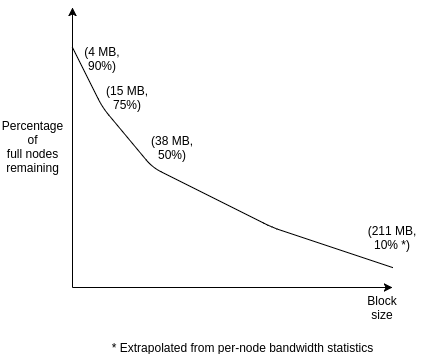
\includegraphics[width=3in]{blocksize_fullnodes.png} }%
%\hfill
%\subcaptionbox{Subcaption B}{ 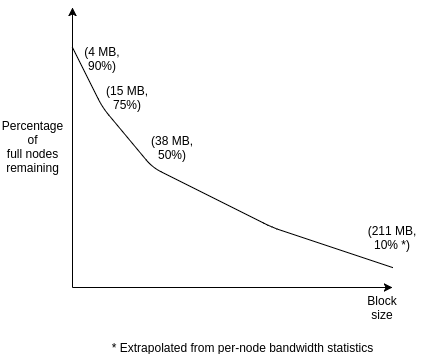
\includegraphics[width=3in]{blocksize_fullnodes.png} }%
%\caption{Caption}
%\end{figure}




\section{The Full Ethereum Gas Function}
\label{appendix:gasfunction}
\todo{Put the full gas function here.}


\end{document}
  
  
  
  
         

        